\chapter{Metodologia}
\label{chap:metodologia}

Este projeto utiliza dados previamente coletados pelo laboratório ao qual faço parte, envolvendo medidas de eletroencefalograma (EEG) e eletromiografia (EMG) de atletas profissionais de basquetebol feminino. O objetivo central deste estudo é investigar a sincronicidade cérebro-corpo e avaliar o impacto da estimulação transcraniana por corrente contínua de alta definição (HD-tDCS) no desempenho atlético durante arremessos de lance livre.

\section{Participantes e Coleta de Dados}

O estudo foi aprovado pelo Comitê de Ética em Pesquisa da UFABC (protocolo: 08070819.1.0000.5594) e conduzido em conformidade com os princípios éticos estabelecidos pela Declaração de Helsinque para experimentos envolvendo seres humanos. Todas as participantes assinaram o Termo de Consentimento Livre e Esclarecido (TCLE) antes de iniciarem sua participação.

As participantes eram consideradas atletas de elite, com um regime de treinamento superior a 10 horas semanais, e foram selecionadas com base em critérios rigorosos:
\begin{itemize}
    \item Participação regular no programa de treinamento da equipe;
    \item Ausência de doenças ou lesões que pudessem interferir na execução do protocolo;
    \item Assinatura do Termo de Consentimento Livre e Esclarecido (TCLE).
\end{itemize}

A amostra foi caracterizada por meio da mensuração de massa corporal, estatura e coleta de informações detalhadas, como nome, data de nascimento, categoria, experiência esportiva, posição no time, fase da temporada, membro dominante e estilo de arremesso. Contudo, devido a problemas técnicos durante a coleta de dados, apenas os dados de 7 atletas foram utilizados nas análises \cite{moscaleski2022}.

Embora o tamanho reduzido da amostra possa ser considerado uma limitação, ele é uma característica comum em estudos que envolvem populações específicas e de difícil acesso, como atletas de elite. Estudos prévios, como o de Boukrina et al. \cite{boukrina2020}, destacam que, em situações em que o aumento do tamanho da amostra não é viável, estratégias como a homogeneidade da amostra e análises que considerem a variabilidade individual podem proporcionar resultados robustos e significativos.

\section{Delineamento Experimental}

O delineamento experimental seguiu um modelo randomizado, cruzado e duplo-cego, amplamente utilizado em estudos de neurociência aplicada e psicofisiologia para minimizar viés e garantir a validade dos resultados. Esse modelo permitiu que todas as participantes fossem expostas tanto à condição de estimulação catódica (HD-tDCS) quanto à condição sham (simulada), aumentando a robustez das comparações intraindividuais.

\begin{figure}[htb]
    \centering
    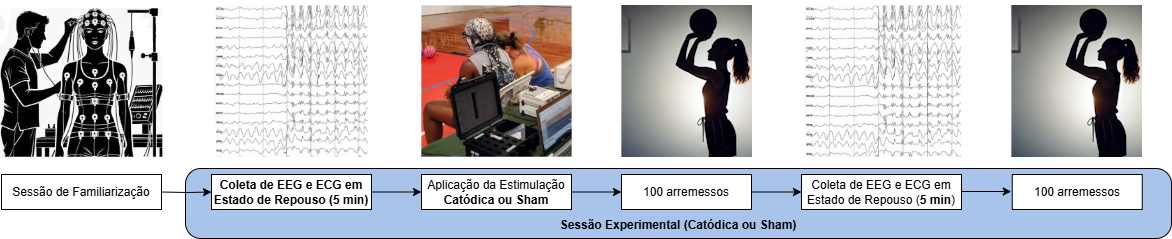
\includegraphics[width=0.9\textwidth]{figs/0_intro_e_desenho_experimental/desenho_experimental_drawio.png}
    \caption{Fluxo do protocolo experimental, incluindo a sessão de familiarização, as duas sessões experimentais (com estimulação catódica ou sham), as coletas de EEG/ECG em repouso e a execução de 200 arremessos por sessão.}
    \label{fig:desenho_experimental}
\end{figure}

Antes das sessões experimentais, foi realizada uma sessão de familiarização, na qual as participantes receberam explicações sobre os objetivos, procedimentos, riscos e benefícios do estudo, além de um período de adaptação ao protocolo experimental. Essa familiarização assegurou que todas estivessem confortáveis com os procedimentos e equipamentos utilizados.

As sessões experimentais ocorreram entre janeiro e fevereiro de 2020, com a seguinte estrutura:
\begin{itemize}
    \item \textbf{Sessão 1}: Familiarização com dispositivos e procedimentos do estudo.
    \item \textbf{Sessões 2 e 3}: Protocolo experimental com 200 arremessos por sessão, totalizando 400 arremessos por atleta.
\end{itemize}

As sessões foram realizadas no mesmo local e horário do treinamento habitual das atletas, garantindo a padronização das condições ambientais. A ordem das condições experimentais foi atribuída de maneira aleatória para cada participante, conforme o modelo cruzado.

\section{Questionários e Escalas}
Além das medidas neurofisiológicas, foram aplicados questionários para avaliar aspectos subjetivos relacionados ao desempenho das atletas. Entre os instrumentos utilizados, destacam-se:
\begin{itemize}
    \item \textbf{Escala de Qualidade Total de Recuperação (TQR)}: avalia o estado geral de recuperação física e mental, fornecendo insights sobre como as participantes se sentem prontas para enfrentar novas atividades físicas após as sessões experimentais;
    \item \textbf{Escala de Percepção Subjetiva de Esforço (PSE)}: mede o esforço percebido pelas participantes ao final de cada sessão experimental, permitindo relacionar o desempenho físico ao nível de fadiga subjetiva;
    \item \textbf{Sport Competition Anxiety Test (SCAT)}: identifica os níveis de ansiedade competitiva das participantes, avaliando como essa variável psicológica pode influenciar a execução das tarefas motoras propostas;
    \item \textbf{Questionário de Motivação Relacionado ao Exercício}: investiga os fatores motivacionais das participantes durante o experimento, analisando seu impacto no engajamento e na qualidade do desempenho.
\end{itemize}
Esses instrumentos permitiram uma análise detalhada de variáveis psicológicas complementares às medidas fisiológicas coletadas, contribuindo para uma visão integrada da sincronicidade cérebro-corpo no desempenho esportivo.


\section{Estimulação Transcraniana por Corrente Contínua de Alta Definição (HD-tDCS)}

A HD-tDCS foi realizada com um estimulador digital MxN da Soterix Medical, utilizando eletrodos Ag/AgCl posicionados em uma touca de EEG. O posicionamento dos eletrodos seguiu um protocolo padronizado baseado em modelagem computacional, garantindo precisão e focalidade na estimulação \cite{datta2008}. 

Foram aplicadas duas condições experimentais: estimulação catódica (ativa) e sham (simulada), com as participantes expostas a ambas em sessões diferentes, de forma cruzada e randomizada. A calibração dos equipamentos foi realizada antes de cada sessão para assegurar a qualidade e a confiabilidade dos dados registrados.

\subsection{Processamento e Análise de Dados}

O processamento e análise dos dados seguiram um fluxo estruturado que abrange desde a coleta e organização dos arquivos até a extração de métricas de sincronização e a aplicação de testes estatísticos para avaliar as diferenças entre condições experimentais. A Figura~\ref{fig:fluxo_processamento} apresenta um diagrama geral dessas etapas.

\begin{figure}[htb]
    \centering
    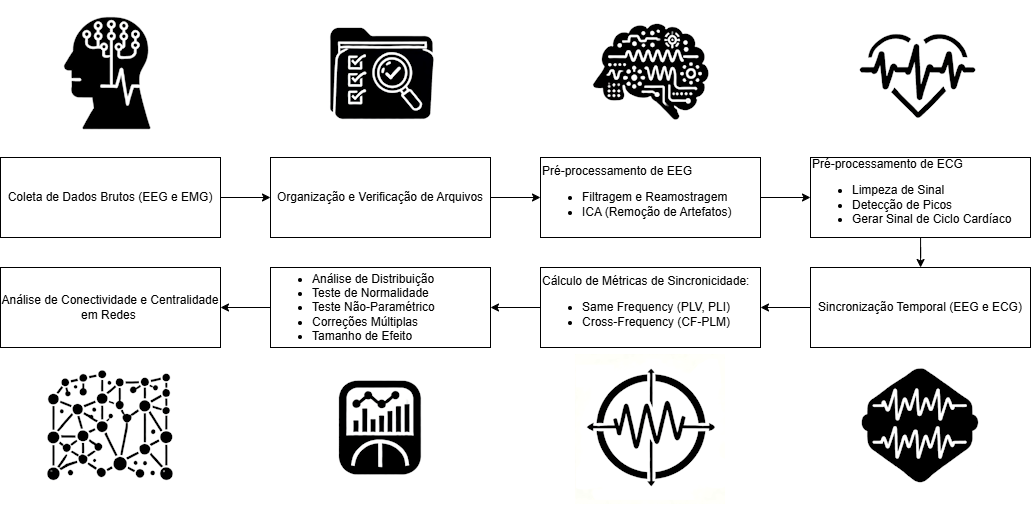
\includegraphics[width=0.9\textwidth]{figs/0_intro_e_desenho_experimental/diagrama_processamento_e_analise_drawio.png}
    \caption{Fluxo geral de processamento e análise de dados, desde a coleta e organização dos arquivos, passando pelas etapas de pré-processamento (EEG e ECG), sincronização temporal, extração de métricas de sincronização (PLI, PLV e CF-PLM) e, por fim, análises estatísticas e de conectividade em rede.}
    \label{fig:fluxo_processamento}
\end{figure}

\subsubsection{Pré-processamento de Dados}
Os sinais de EEG e EMG foram submetidos a etapas de pré-processamento, como filtragem de ruídos e remoção de artefatos por meio de Independent Component Analysis (ICA). Além disso, os sinais de ECG passaram por processos de detecção de picos e extração do ciclo cardíaco. Essas etapas garantiram a qualidade e consistência dos dados analisados.

\subsubsection{Sincronização de Sinais}
Para permitir uma análise integrada, os sinais de EEG e ECG foram alinhados temporalmente, garantindo que as medidas extraídas estivessem sincronizadas e pudessem ser comparadas corretamente. Esse procedimento assegurou a compatibilidade entre os dados das diferentes modalidades.

\subsubsection{Cálculo de Sincronização Funcional}
A sincronização entre os sinais foi avaliada utilizando diferentes métricas. O Phase Locking Value (PLV) e o Phase Lag Index (PLI) foram aplicados para quantificar a conectividade em uma mesma frequência, enquanto a Cross-Frequency Phase Linearity Measurement (CF-PLM) foi utilizada para avaliar acoplamento entre frequências distintas. Antes de sua aplicação nos dados experimentais, esses métodos foram testados e validados por meio de sinais simulados.

\subsubsection{Análise Estatística}
Para investigar diferenças entre condições experimentais, aplicamos métodos estatísticos robustos, incluindo testes de normalidade, testes não-paramétricos e correções para comparações múltiplas. Adicionalmente, utilizamos medidas de centralidade em redes para avaliar a conectividade funcional entre diferentes regiões corticais. Os padrões de conectividade foram representados por meio de gráficos e redes, facilitando a visualização dos resultados.

Esse fluxo sistemático permitiu uma abordagem rigorosa para explorar a sincronicidade cérebro-corpo e avaliar o impacto da estimulação transcraniana no desempenho atlético.
